% !TEX encoding = UTF-8 Unicode
% !TEX root = ../thesis.tex

\begin{figure}[t]	
%	\includegraphics[width=\columnwidth]{fig/quant/quant_visualization}
    \centering
	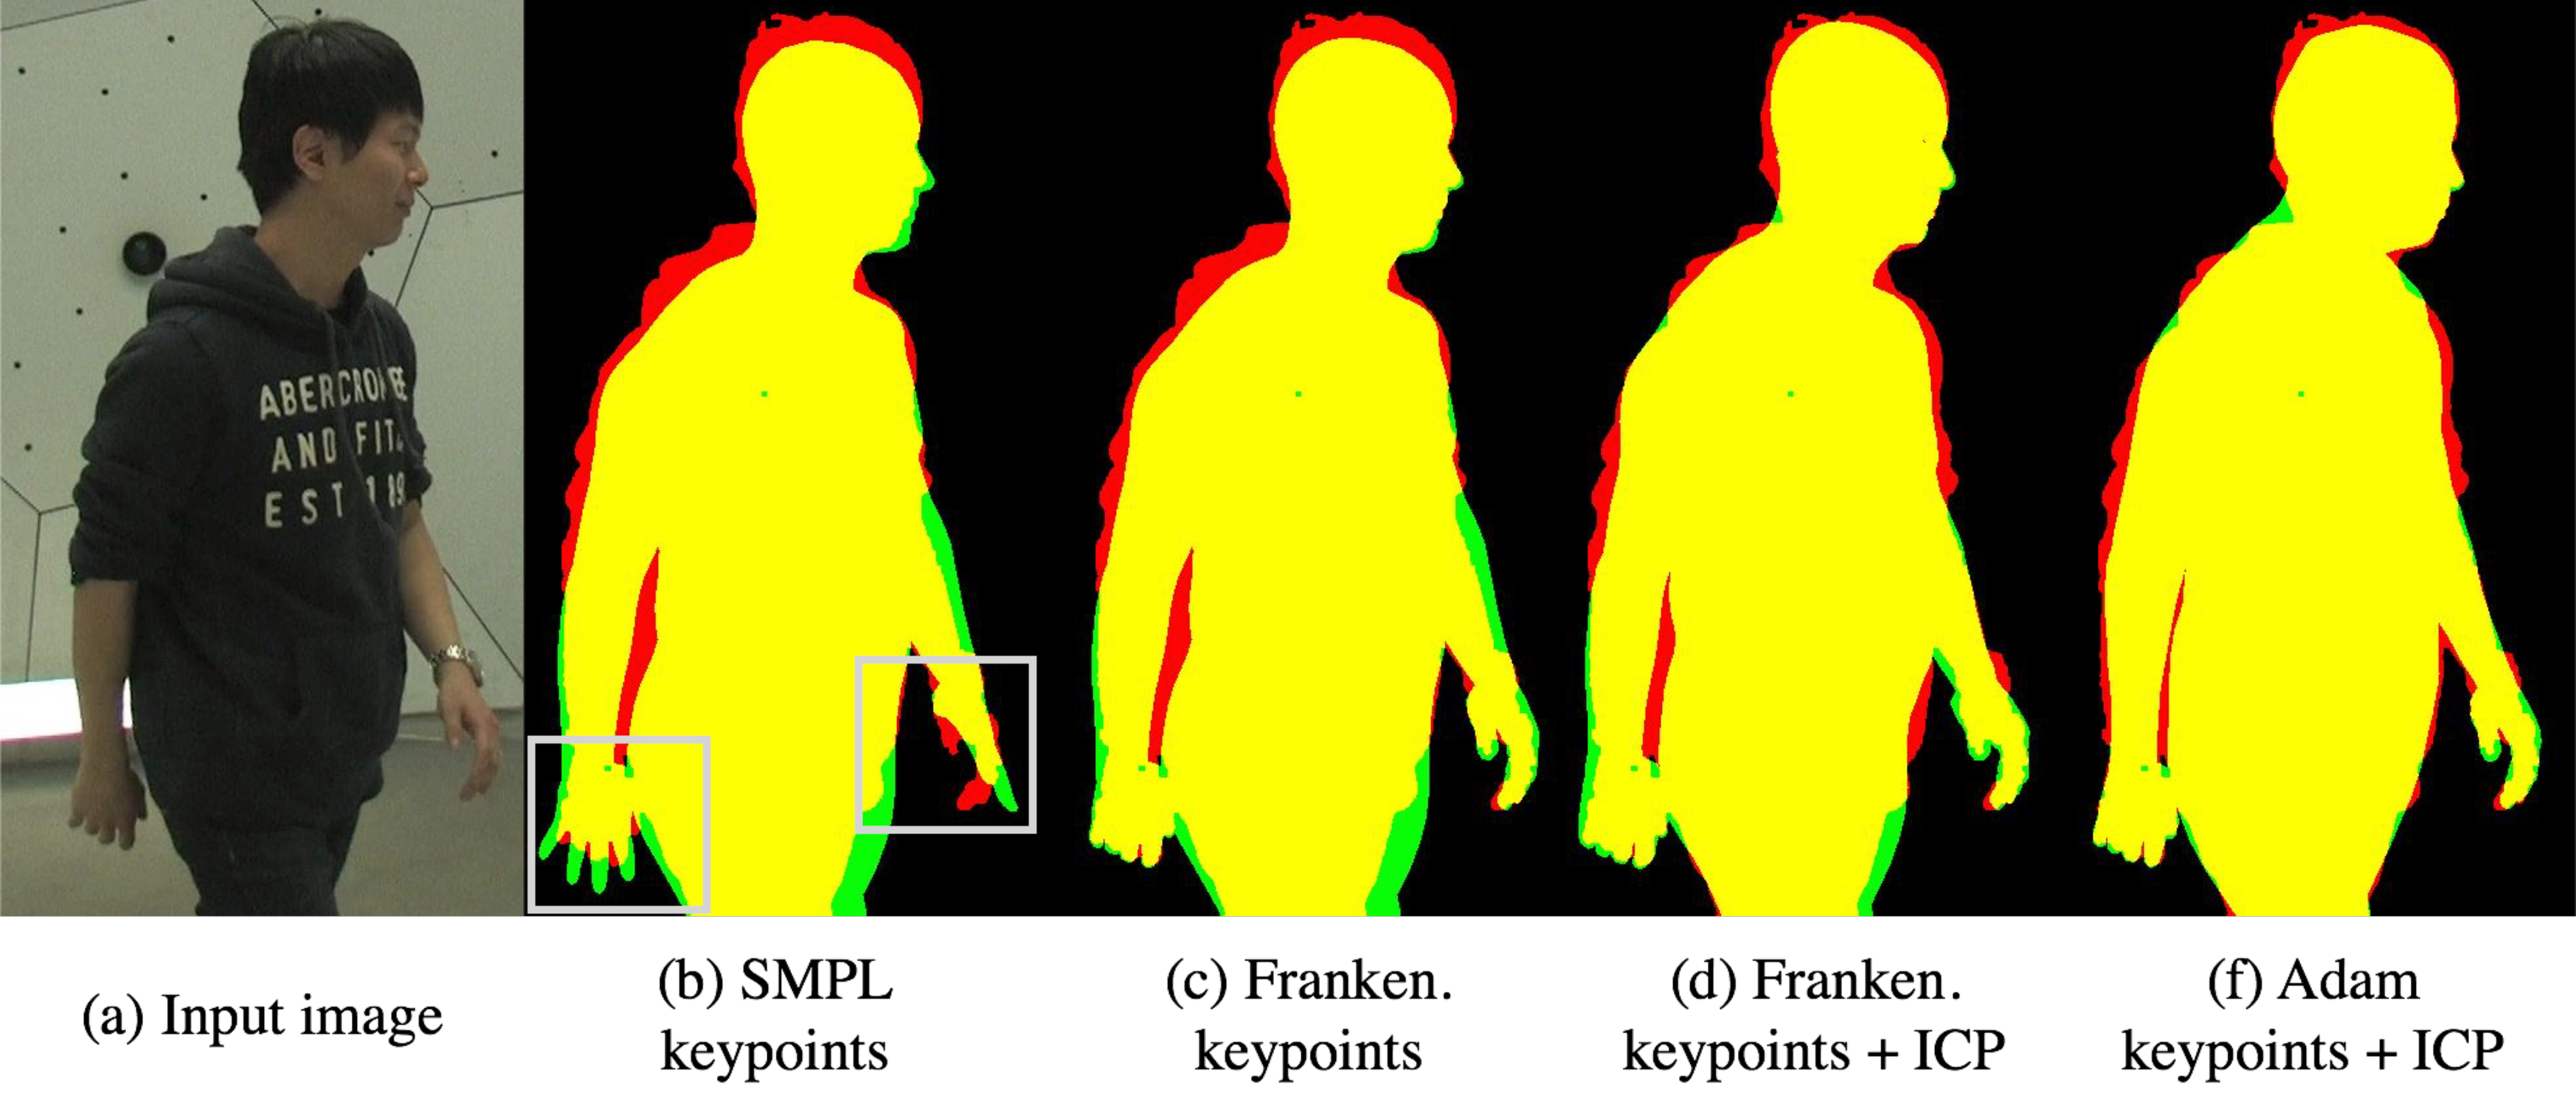
\includegraphics[width=\columnwidth]{tbc_figures/quant_vis_legend}
	%\includegraphics[width=0.9\columnwidth]{fig/quant/silhoutte_quant_final_1115_2am}
	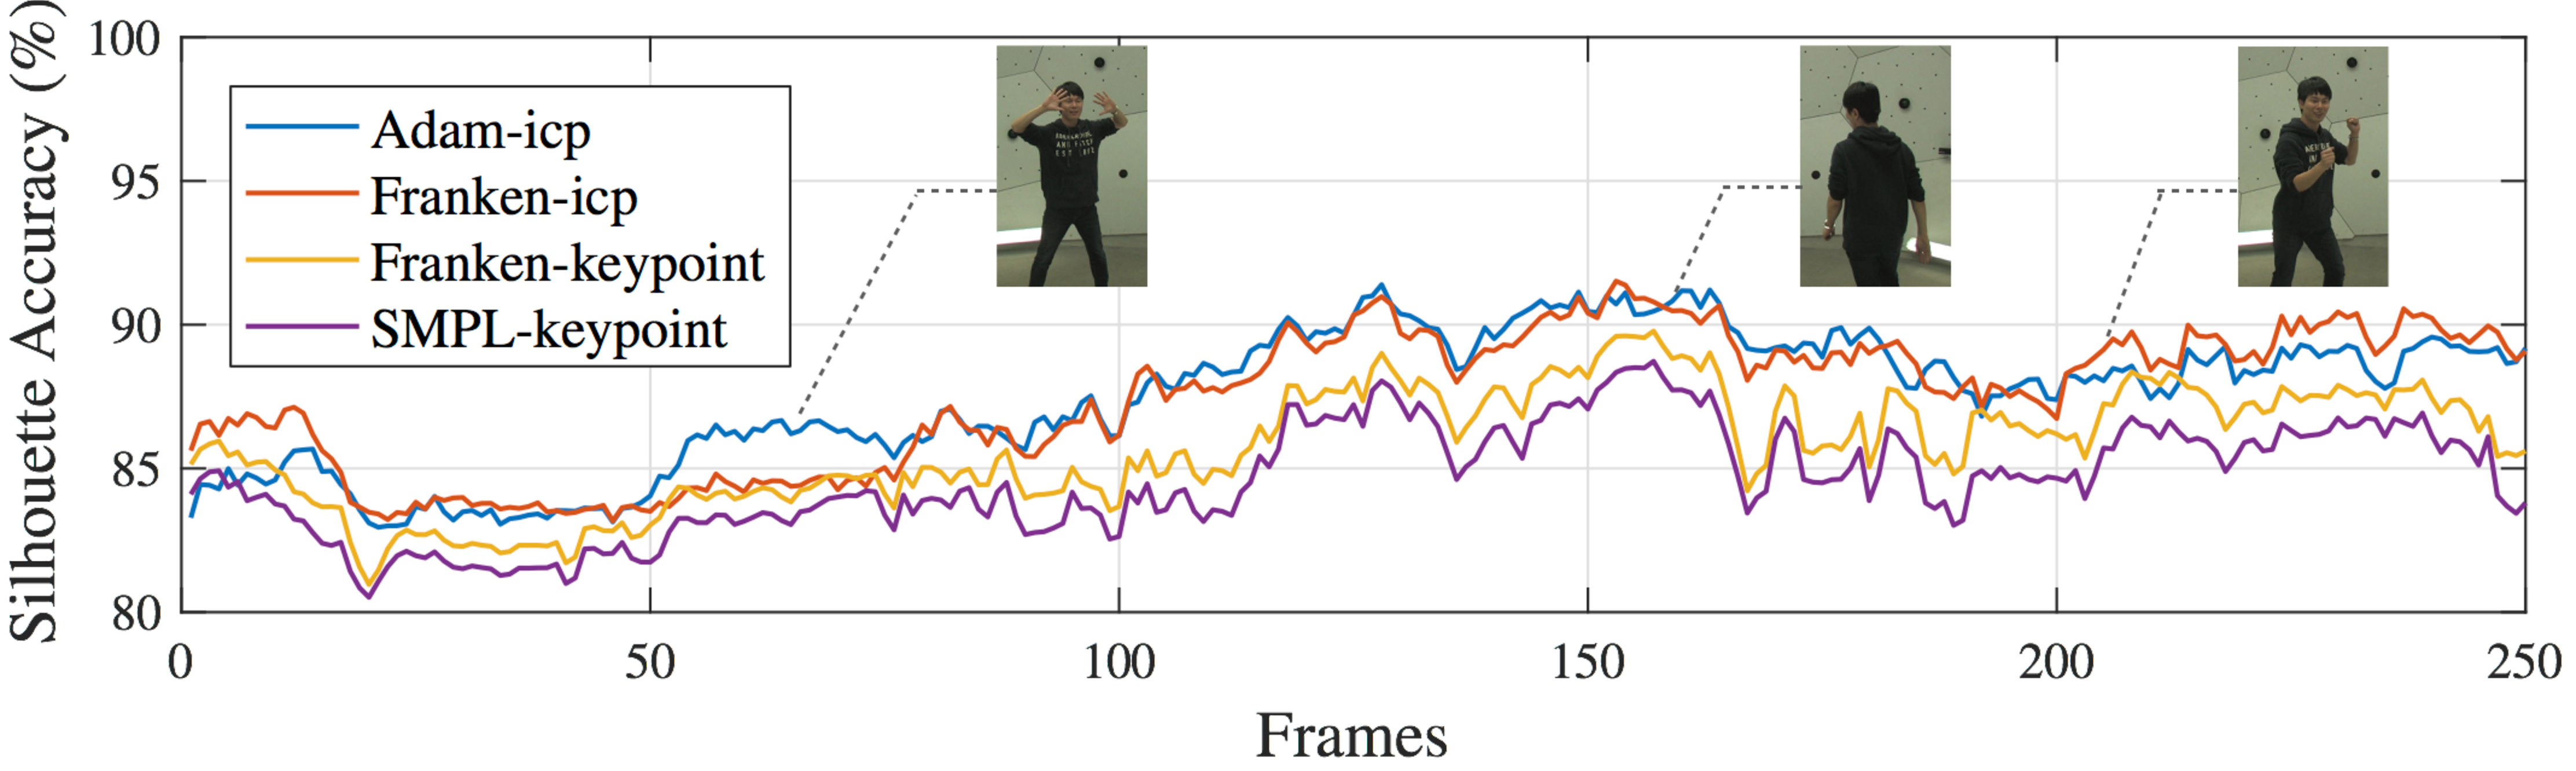
\includegraphics[width=\columnwidth]{tbc_figures/quant_withFigures}
	\caption{(Top) The silhouette from different methods overlayed with ground-truth. The ground truth is drawn in the red channel and the rendered silhouette masks from each model are drawn in the green channel. Thus, the correctly overlapped region is shown as yellow color. (Bottom) Silhouette accuracy compared to the ground truth silhouette.}
	\label{fig:quant_silhoutte_vis}
\end{figure}

\begin{table} [t]	
\centering
	\caption{Accuracy of Silhouettes from different models}\label{Table:quant_silhoette}
	\begin{tabular}{c|c|c|c|c}
		\hline 
		& {SMPL\cite{Loper2015}} & {Frank} & {Frank ICP} & {Adam ICP} \tabularnewline
		\hline 
		Mean &  84.79\% & 85.91\% & 87.68\% & 87.74\%  \tabularnewline
		\hline 
		Std.  &  4.55  & 4.57 & 4.53  & 4.18  \tabularnewline
		\hline 
	\end{tabular} 
	\label{table:quant_sillouette}
\end{table}

% \begin{figure}[t]
% 	\includegraphics[width=\columnwidth]{fig/quant/silhoutte_quant_final_1115_2am}
% 	\caption{Silhouette accuracy by the method of each model compared to the ground truth silhouette.}
% 	\label{fig:quant_silhoutte}
% \end{figure}

% Zoom into hands and faces

\begin{figure*}[t]
	%\includegraphics[width=\textwidth]{qualitativeResults3}
	%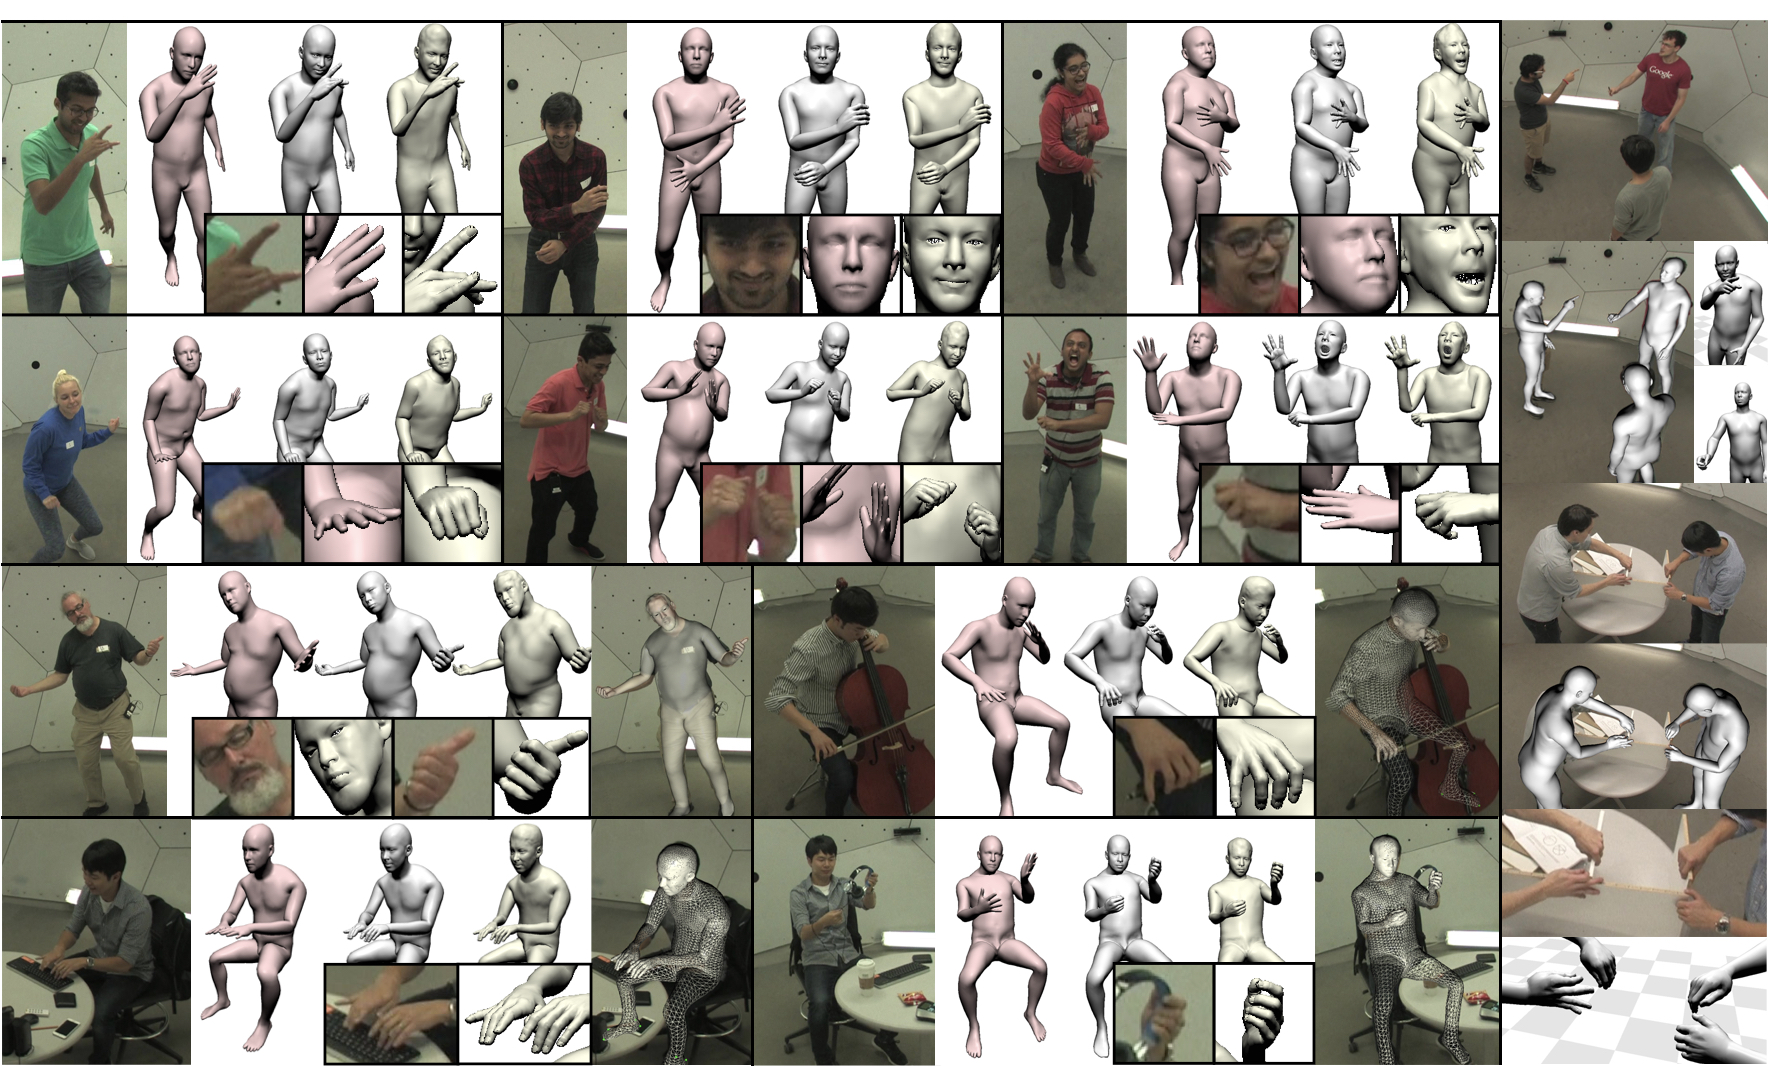
\includegraphics[width=\textwidth]{tbc_figures/Qualitative_180325.jpg}
	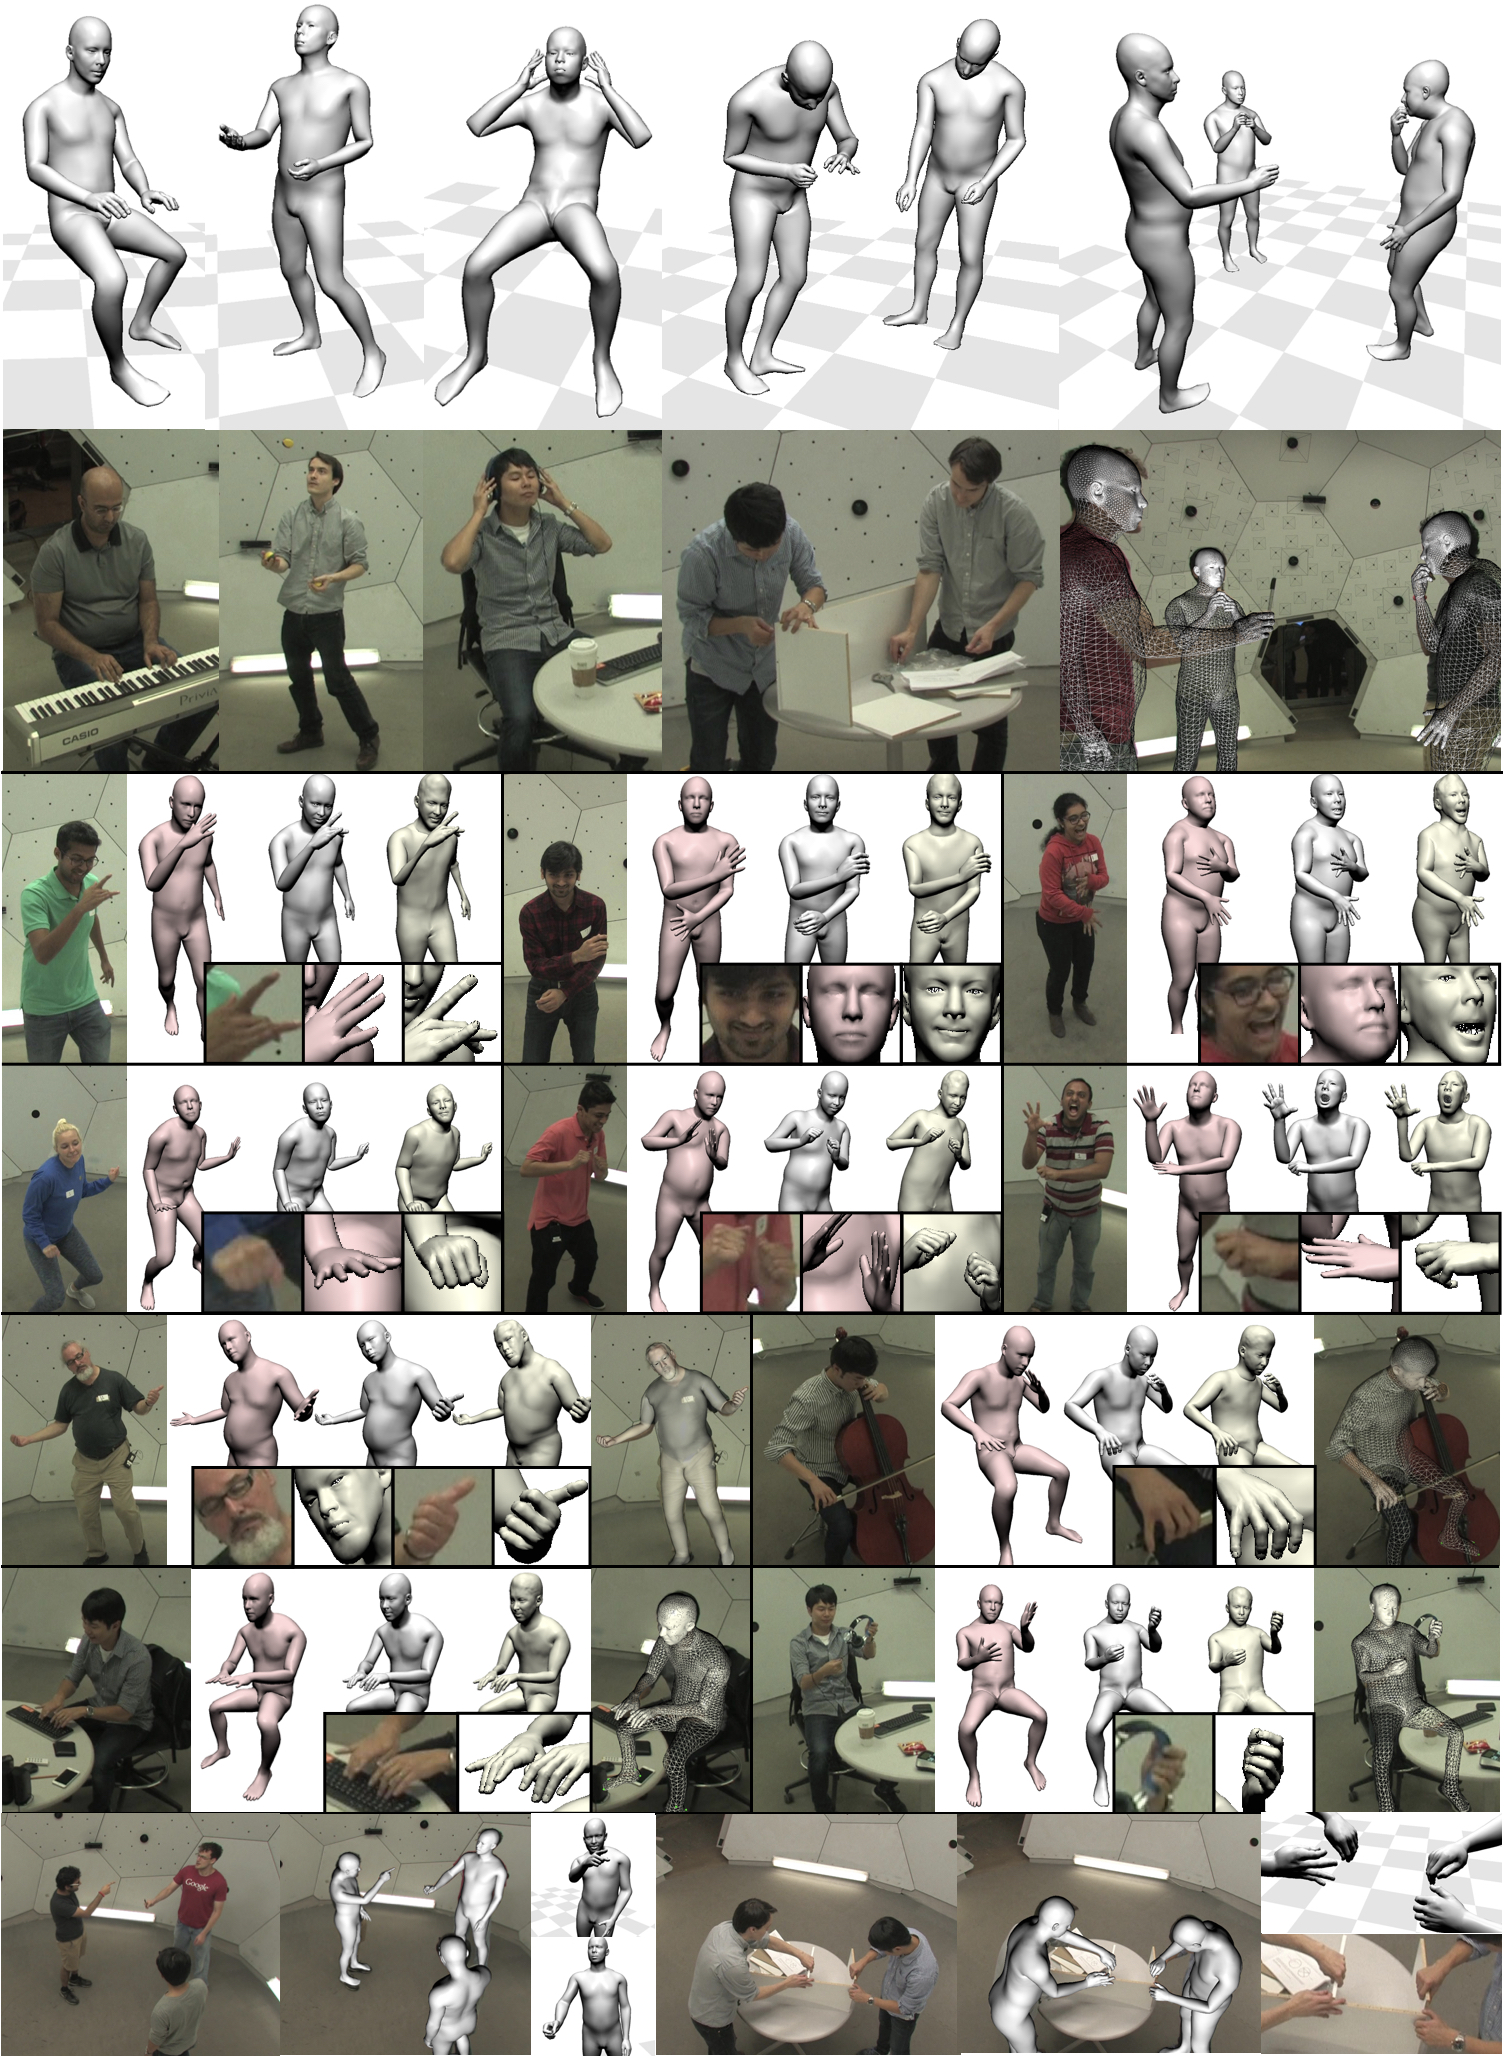
\includegraphics[width=\textwidth]{tbc_figures/Qualitative_thesis.jpg}
	\caption{Total body reconstruction results on various human body motions. For each example scene, the fitting results from three different models are shown by different colors (pink for SMPL~\cite{Loper2015}, silver for Frank, and gold for Adam). 
	%Facial expression and finger gestures captured by our two models provide more realism on the reconstruction output. The Adam model produces more subject-like outputs with simpler parameterization compared to the Frankenstein model.
	}
	\label{fig:qualitativeResults}
\end{figure*}
%

\section{Results}
We perform total motion capture using our two models, Frank and Adam, on various challenging sequences. For experiments, we use the dataset captured in the CMU Panoptic Studio~\cite{Joo-15, joo2017panoptic}. We use 140 VGA cameras to reconstruct 3D body keypoints, 480 VGA cameras for feet, and 31 HD cameras for faces and hands keypoints, and 3D point clouds. We compare the fits produced by our models with the simplified\footnote{In all our comparison, we disabled the pose-dependent blendshapes of SMPL, and thus here SMPL model means the body part of Frank.} SMPL model~\cite{Loper2015}. %In our evaluation, all reconstructions are performed per-frame independently. 

\subsection{Quantitative Evaluation}
% There is no straightforward way to generate ground truth data for total body motion. Thus, we alternatively use ground truth silhouettes in each view as a way to quantify the performance of our method. Since we restrict models in their parameterization space only, this experiment can be considered as a way to quantify the expressive power of each models. To be more reliable, we use silhouettes from 5 different view points. 
We evaluate how well each model can match a moving person by measuring overlap with the ground truth silhouette across 5 different viewpoints for a 10 second sequence. To obtain the ground truth silhouette, we run a background subtraction algorithm using a Gaussian model for the color of each pixel, with post-processing by morphological transforms to remove noise. As an evaluation metric, we compute the percentage of overlap compared to the union between the GT silhouettes and the rendered forground masks after fitting each model. Here, we compare the fitting results of 3 different models: SMPL, our Frank, and our Adam models. The results are shown in Fig.~\ref{fig:quant_silhoutte_vis} and Table~\ref{table:quant_sillouette}. We first compare accuracy between SMPL and Frank model by using only 3D keypoints as measurement cues. The major source of improvement of Frank over SMPL is in the articulated hand model (by construction, the body is almost identical). Including ICP term as cues provides better accuracy. Finally in the comparison between our two models, they show almost similar performance. Ideally we expect Adam to outperform Frank because it has more expressive power for hair and clothing, and it shows better performance for certain body shapes (frame 50-75 in Fig.~\ref{fig:quant_silhoutte_vis}). However, Adam sometimes produces artifacts showing lower accuracy: it tends to generate thinner legs, mainly due to poor 3D point cloud reconstructions in the training data\footnote{Due to dark clothing combined with fewer camera views of the legs.}. However, Adam is simpler for total body motion capture and has potential to be improved once a large dataset is available with a more optimized capture setup.

% \begin{align}
% \frac{\hat{S}_{f}^c\cap S_{f}^c}{\hat{S}_{f}^c \cup S_{f}^c} 
% \label{eq:metric1}
% \end{align}
% where $\hat{S}_{f}^c$ and $S_{f}^c$ are ground truth and rendered silhouettes at frame $f$ and camera $c$. 

%Note that this evaluation is a necessary but not a sufficient condition, because it cannot 
%affected by both shape and motion discrepancy. And it is a necessary condition, not sufficient, because model can be arbitrary deformed or drift inside silhouette.  

%\begin{figure*}[t]
%	\includegraphics[width=\textwidth]{fig/qualitative_group}
%	\caption{Qualitative Results. For each row, (1) an example view; (2) Fitting by only SMPL model; (2) Fitting with Frankenstein model; (3) Fitting with Total model; (4) Other 3D views of the Total model reconstruction.}
%	\label{fig:qualitativeResults_group}
%\end{figure*}

\subsection{Qualitative Results}
We run our method on sequences where face and hand motions naturally occur. The sequences include short range of motion for 70 people used to build Adam, social interactions of multiple people, a furniture building sequence with dexterous hand motions, musical performances (cello and guitars), and commonly observable daily motions such as typing. Most of these sequences are rarely demonstrated in previous markerless motion capture methods since capturing subtle details is key to achieve realism.  Example results are shown in Figure~\ref{fig:qualitativeResults} but are best seen in the accompanying videos. Here, we also qualitatively compare our models (in silver color for Frank, and gold for Adam) with SMPL (without pose-blendshapes, in pink)~\cite{Loper2015}. Note that total body motion capture based on our models produces more realism by capturing subtle details from the hands and faces.


